\chapter{Mutasi dan Keragaman Genetik}\label{ch:g11:mutations}

Seorang anak lahir sama sekali tanpa pigmen --- rambut putih, kulit
pucat, mata yang tidak tahan cahaya terang --- dari dua orang tua biasa
dalam keluarga tanpa riwayat keadaan itu. Sebuah koloni bakteri yang
belum pernah bertemu antibiotik memuat, dari seratus juta \omterm{def:g10:cells-common-unit:cell}{sel},
beberapa yang sudah menahannya. Seorang tukang kebun menemukan satu
cabang semak mawar yang berbunga dengan warna yang berbeda. Pada tiap
hal itu sebuah urutan \omterm{def:g10:universal-dna:information}{DNA} telah berubah, sekali, dalam satu \omterm{def:g10:cells-common-unit:cell}{sel}; dan
pada tiap hal itu perubahannya disalin dengan setia sesudahnya. Bab ini
membahas perubahan itu: apa perubahannya, dari mana asalnya, bagaimana
\omterm{def:g10:cells-common-unit:cell}{selnya} membatasinya, dan mengapa kehidupan bergantung pada perubahan
itu yang tidak pernah benar-benar berhenti.

\section{Apa itu mutasi}

\begin{definition}[Mutasi]\label{def:g11:mutations:mutation}
Sebuah \emph{mutasi}\index{mutasi} adalah perubahan urutan \omterm{def:g10:universal-dna:nucleotide}{nukleotida}
sebuah molekul \omterm{def:g10:universal-dna:information}{DNA}, yang diwariskan kepada keturunan \omterm{def:g10:cells-common-unit:cell}{sel} tempat ia
terjadi. Yang terlazim adalah \emph{mutasi titik}, yang mengenai satu
atau beberapa \omterm{def:g10:universal-dna:nucleotide}{nukleotida}:
\begin{itemize}
  \item \emph{substitusi}: satu \omterm{def:g10:universal-dna:nucleotide}{nukleotida} digantikan yang lain;
  \item \emph{insersi}: satu \omterm{def:g10:universal-dna:nucleotide}{nukleotida} atau lebih ditambahkan;
  \item \emph{delesi}: satu \omterm{def:g10:universal-dna:nucleotide}{nukleotida} atau lebih disingkirkan.
\end{itemize}
Perubahan yang lebih besar --- sebuah ruas yang digandakan, dibalik,
dipindahkan, atau satu \omterm{def:g11:cell-cycle-mitosis:chromosome}{kromosom} utuh yang bertambah atau hilang ---
juga merupakan mutasi.
\end{definition}

\begin{omfigure}
\begin{tikzpicture}[font=\small\ttfamily]
  \tikzset{seq/.style={anchor=west}}
  \node[seq] at (0,0) {asli\ \ \ \ \ \ \ \ \ \ ATG GCT TAC GGA TCC};
  \node[seq] at (0,-0.8) {substitusi\ \ \ \ ATG GCT T\textcolor{omThm}{\textbf{G}}C GGA TCC};
  \node[seq] at (0,-1.6) {insersi\ \ \ \ \ \ \ ATG GCT TA\textcolor{omThm}{\textbf{A}} CGG ATC C};
  \node[seq] at (0,-2.4) {delesi\ \ \ \ \ \ \ \ ATG GCT T\textcolor{omThm}{\textbf{\_}}C GGA TCC};
  \node[seq, font=\small] at (7.9,-0.8) {satu huruf berubah};
  \node[seq, font=\small] at (7.9,-1.6) {satu huruf bertambah: semua yang menyusul bergeser};
  \node[seq, font=\small] at (7.9,-2.4) {satu huruf hilang: semua yang menyusul bergeser};
\end{tikzpicture}

{\small Tiga \omterm{def:g11:mutations:mutation}{mutasi} titik pada urutan yang sama (hurufnya dikelompokkan
bertiga karena alasan yang dijelaskan pada
\cref{ch:g11:gene-expression}). Substitusi mengubah satu kedudukan;
insersi atau delesi menggeser segalanya di hilirnya.}
\end{omfigure}

\begin{proposition}[Di mana mutasi terjadi, dan pada siapa]\label{prop:g11:mutations:where}
\omterm{def:g11:mutations:mutation}{Mutasi} yang terjadi dalam \omterm{def:g10:cells-common-unit:cell}{sel} tubuh (\emph{\omterm{def:g11:mutations:mutation}{mutasi} somatik}) hanya
diteruskan kepada keturunan \omterm{def:g10:cells-common-unit:cell}{sel} itu: paling banyak sebidang jaringan,
pada satu individu. \omterm{def:g11:mutations:mutation}{Mutasi} dalam \omterm{def:g10:cells-common-unit:cell}{sel} kelamin --- sebuah gamet atau
salah satu bakalnya --- diteruskan kepada keturunan yang dikandung
darinya dan kepada setiap \omterm{def:g10:cells-common-unit:cell}{selnya}: \emph{\omterm{def:g11:mutations:mutation}{mutasi} \omterm{def:g10:cells-common-unit:cell}{sel} kelamin} adalah
satu-satunya macam yang masuk ke pewarisan sifat \omterm{def:g10:biodiversity-scales:species}{spesiesnya}. Cabang
ganjil semak mawarnya bersifat somatik; keadaan anak tanpa pigmen itu
berasal dari \omterm{def:g11:mutations:mutation}{mutasi} \omterm{def:g10:cells-common-unit:cell}{sel} kelamin pada seorang moyangnya, yang terbawa
diam-diam selama beberapa keturunan.
\end{proposition}
\admitted

\begin{example}[Frekuensi mutasinya]\label{ex:g11:mutations:frequency}
Replikasi meninggalkan sekitar satu kesalahan tiap $10^9$ \omterm{def:g10:universal-dna:nucleotide}{nukleotida}
(\cref{ch:g11:dna-replication}). Karena itu \omterm{def:g10:universal-dna:gene}{gen} sepanjang $\num{3000}$
pasangan \omterm{def:g10:universal-dna:nucleotide}{basa} salah disalin sekitar sekali tiap $\num{300000}$
replikasi; seorang manusia, yang genomnya disalin sekitar $10^{16}$
kali seumur hidup, menumpuk \omterm{def:g11:mutations:mutation}{mutasi} pada tiap \omterm{def:g10:universal-dna:gene}{gen} dalam banyak \omterm{def:g10:cells-common-unit:cell}{sel}. Tiap
anak lahir dengan sekitar 60 \omterm{def:g11:mutations:mutation}{mutasi} baru yang tidak dibawa kedua orang
tuanya --- hampir semuanya dalam 98\% genomnya yang bukan \omterm{def:g10:universal-dna:gene}{gen}.
\end{example}

\section{Sebabnya: spontan dan terimbas}

\begin{proposition}[Mutasi spontan]\label{prop:g11:mutations:spontaneous}
\omterm{def:g11:mutations:mutation}{Mutasi} muncul dalam setiap \omterm{def:g10:cells-common-unit:cell}{sel}, tanpa perantara luar apa pun: dari
pemasangan keliru yang langka yang lolos dari pemeriksaan polimerasenya,
dan dari ketakmantapan kimia \omterm{def:g10:universal-dna:information}{DNA} itu sendiri, yang \omterm{def:g10:universal-dna:nucleotide}{basanya} dirusak
ribuan kali sehari tiap \omterm{def:g10:cells-common-unit:cell}{sel} oleh air dan molekul reaktif \omterm{def:g10:cell-metabolism:metabolism}{metabolisme}
biasa. \emph{\omterm{def:g11:mutations:mutation}{Mutasi} spontan} semacam itu bersifat \emph{acak}: ia
terjadi pada kedudukan mana pun, dengan laju yang tidak bergantung pada
apakah perubahannya akan berguna bagi \omterm{def:g10:cells-common-unit:cell}{selnya}.
\end{proposition}
\begin{proof}[Bukti percobaan]
Lederberg (1952) menyebarkan bakteri yang belum pernah terpapar
antibiotik pada sebuah cawan, membiarkannya tumbuh menjadi koloni, lalu
menekankan bantalan beludru pada cawannya dan mencapkan bekasnya ---
koloni yang sama pada kedudukan yang sama --- pada beberapa cawan yang
memuat antibiotik. Segelintir koloni yang tahan muncul pada
\emph{kedudukan yang sama} pada tiap cawan antibiotiknya. Karena
koloni itu berasal dari koloni yang sama pada cawan aslinya, yang
belum pernah bertemu antibiotik, \omterm{def:g11:mutations:mutation}{mutasi} ketahanannya sudah ada sebelum
paparannya: antibiotiknya menyingkapkannya dan tidak menyebabkannya.
\omterm{def:g11:mutations:mutation}{Mutasinya} terjadi secara acak selama pertumbuhan koloninya, tanpa
mengindahkan kegunaannya kelak.
\end{proof}

\begin{omfigure}
\begin{tikzpicture}[font=\small, >=Stealth]
  \tikzset{plate/.style={draw, thick, circle, minimum size=2.4cm, fill=omDef!6}}
  \node[plate] (p0) at (0,0) {};
  \foreach \x/\y in {-0.6/0.5, 0.3/0.7, -0.2/-0.2, 0.7/-0.1, -0.7/-0.6, 0.4/-0.7, 0.0/0.25, -0.35/0.85}
    \fill[omDef!60] (\x,\y) circle (2.2pt);
  \fill[omThm] (0.3,0.7) circle (2.6pt); \fill[omThm] (-0.7,-0.6) circle (2.6pt);
  \node[anchor=north, align=center] at (0,-1.35) {cawan asli,\\ tanpa antibiotik};
  \node[draw, fill=gray!25, minimum width=2.4cm, minimum height=0.35cm] (v) at (3.6,0) {beludru};
  \draw[->, thick] (1.3,0) -- (v.west);
  \node[plate, fill=omProp!8] (p1) at (7.0,1.5) {};
  \node[plate, fill=omProp!8] (p2) at (7.0,-1.5) {};
  \draw[->, thick] (v.east) -- (5.7,1.2);
  \draw[->, thick] (v.east) -- (5.7,-1.2);
  \fill[omThm] (7.3,2.2) circle (2.6pt); \fill[omThm] (6.3,0.9) circle (2.6pt);
  \fill[omThm] (7.3,-0.8) circle (2.6pt); \fill[omThm] (6.3,-2.1) circle (2.6pt);
  \node[anchor=west, align=left] at (8.3,1.5) {cawan berantibiotik:\\ dua kedudukan yang sama};
  \node[anchor=west, align=left] at (8.3,-1.5) {cawan berantibiotik:\\ dua kedudukan yang sama};
\end{tikzpicture}

{\small Penanaman replika. Koloni yang tumbuh tanpa antibiotik dicapkan
pada cawan berantibiotik. Koloni yang tahan (merah) muncul pada
kedudukan yang serupa pada tiap replikanya: ketahanannya sudah ada
dalam koloni aslinya, sebelum sentuhan apa pun dengan obatnya.}
\end{omfigure}

\begin{definition}[Mutagen]\label{def:g11:mutations:mutagen}
Sebuah \emph{mutagen}\index{mutagen} adalah perantara ragawi atau kimia
yang menaikkan laju \omterm{def:g11:mutations:mutation}{mutasi} dengan merusak \omterm{def:g10:universal-dna:information}{DNA}. Cahaya ultraviolet
melaskan timin yang bertetangga pada satu untai; sinar-X dan
keradioaktifan memutuskan untainya; zat kimia seperti benzopiren asap
tembakau atau aflatoksin biji-bijian berjamur menempel pada \omterm{def:g10:universal-dna:nucleotide}{basanya} dan
memuntir heliksnya. \omterm{def:g10:cells-common-unit:cell}{Sel} yang terpapar mutagen membawa \emph{\omterm{def:g11:mutations:mutation}{mutasi}
terimbas} di samping \omterm{def:g11:mutations:mutation}{mutasi} spontannya --- tetap pada kedudukan yang
acak, hanya lebih banyak jumlahnya.
\end{definition}

\begin{example}[Ultraviolet pada ragi]\label{ex:g11:mutations:uv}
\omterm{def:g10:cells-common-unit:cell}{Sel} ragi disebarkan pada cawan dan dipaparkan pada cahaya ultraviolet
selama waktu yang meningkat: setelah \qty{10}{s} separuh \omterm{def:g10:cells-common-unit:cell}{selnya} gagal
membentuk koloni, setelah \qty{20}{s} seperempatnya, setelah
\qty{30}{s} seperdelapannya --- tiap dosisnya membagi dua yang selamat.
Di antara yang selamat, bagian koloni dengan sifat yang berubah secara
kasatmata (warna, bentuk, ketidakmampuan tumbuh pada gula tertentu)
naik dari satu tiap sejuta menjadi satu tiap seribu. Lampunya membunuh
dengan merusak \omterm{def:g10:universal-dna:information}{DNA} melampaui perbaikannya, dan memutasi dengan
merusaknya tepat sebelum batas itu.
\end{example}

\begin{omfigure}
\begin{tikzpicture}
\begin{axis}[
  width=0.86\linewidth, height=5.6cm,
  axis x line=bottom, axis y line=left,
  xmin=0, xmax=65, ymin=0, ymax=110,
  xlabel={paparan ultraviolet (s)}, ylabel={yang selamat (\%)},
  xlabel style={font=\small, at={(axis description cs:0.5,-0.12)}, anchor=north},
  ylabel style={font=\small},
  tick label style={font=\small}, xtick={0,10,20,30,40,50,60}, ytick={0,25,50,75,100},
  legend style={at={(0.97,0.95)}, anchor=north east, font=\small, draw=none},
  legend cell align=left,
]
\addplot[thick, omDef, mark=*, mark size=1.5pt] coordinates
  {(0,100) (10,50) (20,25) (30,12.5) (40,6.3) (50,3.1) (60,1.6)};
\addplot[thick, omThm, dashed, mark=square*, mark size=1.5pt] coordinates
  {(0,100) (10,10) (20,1) (30,0.1) (40,0.01)};
\legend{ragi normal, ragi tanpa enzim perbaikan}
\end{axis}
\end{tikzpicture}

{\small Ketahanan hidup \omterm{def:g10:cells-common-unit:cell}{sel} ragi terhadap paparan ultraviolet. \omterm{def:g10:cells-common-unit:cell}{Sel}
normal kehilangan separuh jumlahnya tiap \qty{10}{s}; galur yang tidak
mampu memperbaiki kerusakan ultraviolet kehilangan sembilan
persepuluhnya tiap \qty{10}{s}. Bedanya adalah hasil kerja perbaikannya.}
\end{omfigure}

\begin{omfigure}
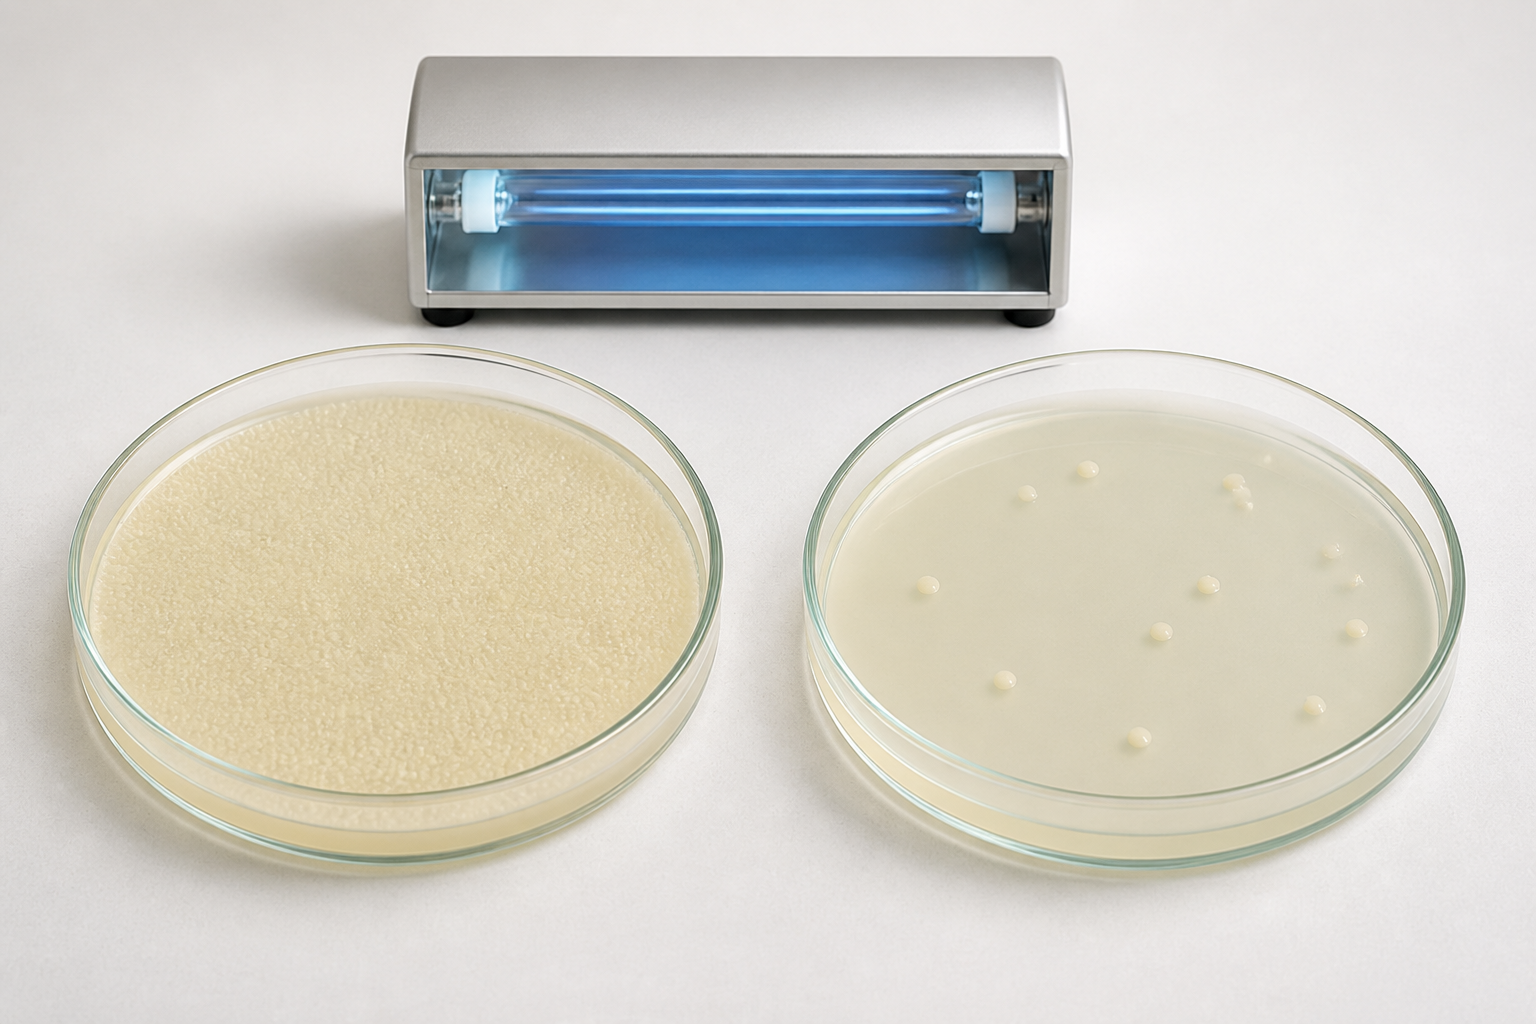
\includegraphics[width=0.6\linewidth]{images/book2/ai/g11-mutation-uv-plates.png}

{\small Dua cawan yang ditanami bakteri yang sama. Kiri: tanpa paparan,
sebuah hamparan yang menerus. Kanan: setelah paparan ultraviolet, hanya
\omterm{def:g10:cells-common-unit:cell}{sel} yang kerusakan \omterm{def:g10:universal-dna:information}{DNA-nya} terperbaiki tepat waktu yang tumbuh menjadi koloni.}
\end{omfigure}

\section{Sel melawan: perbaikan}

\begin{proposition}[Perbaikan DNA]\label{prop:g11:mutations:repair}
Sebuah \omterm{def:g10:cells-common-unit:cell}{sel} menderita puluhan ribu lesi \omterm{def:g10:universal-dna:information}{DNA} sehari dan hampir tidak
menyimpan satu pun: sistem \omterm{def:g10:cell-metabolism:metabolism}{enzim} khusus meronda \omterm{prop:g10:universal-dna:helix}{heliks gandanya},
mengenali \omterm{def:g10:universal-dna:nucleotide}{basa} yang rusak atau salah pasang, memotong keluar ruas yang
cacat pada satu untai dan membangunnya kembali dengan memakai untai
yang lain sebagai cetakan --- yaitu \omterm{prop:g10:universal-dna:helix}{komplementaritas}
\cref{ch:g10:universal-dna} sekali lagi. Sebuah lesi menjadi \omterm{def:g11:mutations:mutation}{mutasi}
hanya jika ia lolos dari perbaikan sebelum replikasi berikutnya
menyalinnya. Perbaikan itulah sebabnya laju \omterm{def:g11:mutations:mutation}{mutasinya} $10^{-9}$ dan
bukan $10^{-5}$.
\end{proposition}
\begin{proof}[Bukti percobaan]
Orang dengan keadaan turunan xeroderma pigmentosum tidak punya salah
satu \omterm{def:g10:cell-metabolism:metabolism}{enzim} yang memotong keluar kerusakan ultraviolet. Kulitnya, jika
terpapar cahaya siang biasa, menumbuhkan kanker seribu kali lebih
sering daripada kulit normal dan sejak masa kanak-kanak awal; jika
terlindung dari matahari, kulitnya normal. Ultraviolet yang sama, lesi
yang sama --- tetapi tanpa perbaikannya lesinya tinggal, dan \omterm{def:g11:mutations:mutation}{mutasinya}
menumpuk dalam \omterm{def:g10:universal-dna:gene}{gen} yang mengendalikan pembelahan \omterm{def:g10:cells-common-unit:cell}{sel}
(\cref{ch:g11:cancer}). Galur ragi dan bakteri yang tidak punya \omterm{def:g10:cell-metabolism:metabolism}{enzim}
perbaikan memperlihatkan kepekaan berlebih yang sama di laboratorium.
\end{proof}

\begin{omfigure}
\begin{tikzpicture}[font=\small, >=Stealth,
  b/.style={draw, rounded corners, align=center, text width=2.6cm, minimum height=1.1cm}]
  \node[b, fill=omProp!15] (a) at (0,0) {ultraviolet melaskan\\ dua T yang bersebelahan};
  \node[b, fill=omDef!12] (bx) at (3.4,0) {enzim perbaikan\\ mengenali puntirannya};
  \node[b, fill=omDef!12] (c) at (6.8,0) {ruas yang rusak\\ dipotong dari satu untai};
  \node[b, fill=omDef!12] (d) at (10.2,0) {celahnya diisi ulang\\ memakai untai yang utuh};
  \draw[->] (a) -- (bx); \draw[->] (bx) -- (c); \draw[->] (c) -- (d);
  \node[b, fill=omThm!12] (e) at (3.4,-2.0) {replikasi menyalin\\ lesinya};
  \node[b, fill=omThm!12] (f) at (6.8,-2.0) {sebuah mutasi, kini\\ menetap};
  \draw[->] (a.south) |- node[pos=0.25, left, font=\scriptsize, align=right] {jika tak terperbaiki\\ tepat waktu} (e.west);
  \draw[->] (e) -- (f);
\end{tikzpicture}

{\small Perlombaan antara perbaikan dan replikasi. Lesi yang dipotong
keluar dan dibangun kembali dari untai yang lain tidak meninggalkan
jejak; lesi yang masih ada ketika garpunya lewat disalin ke dalam
urutannya dan menjadi \omterm{def:g11:mutations:mutation}{mutasi}.}
\end{omfigure}

\section{Akibat sebuah mutasi}

\begin{proposition}[Dari urutan ke fenotipe]\label{prop:g11:mutations:consequences}
Sebuah \omterm{def:g11:mutations:mutation}{mutasi} mengubah satu \omterm{def:g10:universal-dna:gene}{alel} menjadi \omterm{def:g10:universal-dna:gene}{alel} yang baru. Pengaruhnya
bergantung pada tempat jatuhnya dan pada apa yang diperbuatnya terhadap
\omterm{def:g10:chemistry-of-life:families}{protein} yang disandikan \omterm{def:g10:universal-dna:gene}{gennya} (\cref{ch:g11:gene-expression} memberi
aturannya):
\begin{itemize}
  \item di luar \omterm{def:g10:universal-dna:gene}{gen} mana pun, atau pada kedudukan yang tidak mengubah
        \omterm{def:g10:chemistry-of-life:families}{proteinnya}: \emph{tanpa pengaruh} --- inilah yang terbanyak;
  \item di dalam sebuah \omterm{def:g10:universal-dna:gene}{gen}, yang mengubah satu \omterm{def:g10:chemistry-of-life:families}{asam amino}: \omterm{def:g10:chemistry-of-life:families}{protein}
        yang bekerja sedikit berbeda, atau sama sekali tidak bekerja,
        atau kadang-kadang lebih baik;
  \item di dalam sebuah \omterm{def:g10:universal-dna:gene}{gen}, yang menggeser atau memenggal pesannya:
        lazimnya \omterm{def:g10:chemistry-of-life:families}{protein} yang tidak bekerja.
\end{itemize}
Apakah \omterm{def:g10:chemistry-of-life:families}{protein} yang berubah itu merugikan, netral atau berguna
bergantung pada lingkungannya: \omterm{def:g10:universal-dna:gene}{alel} \omterm{def:g10:universal-dna:gene}{gen} hemoglobin yang sama menjadi
beban di daerah tanpa malaria dan menjadi perlindungan di tempat
malaria hadir.
\end{proposition}
\admitted

\begin{example}[Pigmen yang hilang, pigmen yang tersimpan]\label{ex:g11:mutations:pigment}
Pigmen melanin dibuat sebuah \omterm{def:g10:cell-metabolism:metabolism}{enzim}. Puluhan \omterm{def:g11:mutations:mutation}{mutasi} \omterm{def:g10:universal-dna:gene}{gennya} yang berbeda
telah dikenal, yang masing-masing menghasilkan \omterm{def:g10:cell-metabolism:metabolism}{enzim} yang tidak bekerja
dan, pada orang yang membawa dua \omterm{def:g10:universal-dna:gene}{alel} semacam itu, keadaan tanpa pigmen
pada pembuka bab ini. Setiap satunya muncul secara acak, sekali, dalam
sebuah \omterm{def:g10:cells-common-unit:cell}{sel} kelamin; keadaan yang kasatmata itu muncul hanya ketika dua
pembawa mewariskan \omterm{def:g10:universal-dna:gene}{alelnya} yang diam kepada anak yang sama. \omterm{def:g10:universal-dna:gene}{Gen} yang
sama, dalam \omterm{def:g10:universal-dna:gene}{alel} yang lain, membuat \omterm{def:g10:cell-metabolism:metabolism}{enzim} yang sedikit kurang aktif ---
dan kulit yang lebih terang, yang lazim pada populasi yang selama
ribuan tahun hidup di lintang tinggi, tempat pigmen yang sedikit lebih
sedikit membiarkan kulitnya membuat vitamin D yang lebih banyak dari
matahari yang lemah.
\end{example}

\begin{proposition}[Mutasi, sumber keragaman]\label{prop:g11:mutations:source}
Tiap \omterm{def:g10:universal-dna:gene}{alel} tiap \omterm{def:g10:universal-dna:gene}{gen} bermula sebagai \omterm{def:g11:mutations:mutation}{mutasi} \omterm{def:g10:universal-dna:gene}{alel} yang lebih dahulu.
\omterm{def:g11:mutations:mutation}{Mutasi} adalah satu-satunya proses yang menciptakan \omterm{def:g10:universal-dna:information}{informasi genetik}
yang baru; pengocokan seksual pada tahun terakhir hanya menggabungkan
ulang apa yang telah dibuat \omterm{def:g11:mutations:mutation}{mutasi}. Meskipun langka, acak dan sebagian
besar netral atau merugikan bagi individunya, \omterm{def:g11:mutations:mutation}{mutasi} tetap merupakan
yang memasok, sepanjang beberapa keturunan, keragaman yang menjadi
sandaran evolusi \cref{ch:g10:biodiversity-scales}.
\end{proposition}
\admitted

\begin{method}[Menganalisis sebuah mutasi]\label{met:g11:mutations:analyse}
\begin{enumerate}
  \item Bandingkan urutan mutannya dengan urutan aslinya, huruf demi
        huruf, dan sebutkan nama perubahannya (substitusi, insersi,
        delesi; berapa \omterm{def:g10:universal-dna:nucleotide}{nukleotida}).
  \item Tentukan letaknya: di dalam \omterm{def:g10:universal-dna:gene}{gen} atau di luarnya; jika di dalam
        \omterm{def:g10:universal-dna:gene}{gen}, apakah pembacaan pesannya bergeser.
  \item Kenali \omterm{def:g10:cells-common-unit:cell}{sel} tempatnya terjadi: somatik (satu individu, satu
        jaringan) atau \omterm{def:g10:cells-common-unit:cell}{sel} kelamin (diwariskan).
  \item Carilah sebabnya jika lajunya tidak lazim (paparan \omterm{def:g11:mutations:mutagen}{mutagen},
        perbaikan yang cacat); jika tidak, timpakan pada kebetulan.
  \item Timbanglah akibatnya pada aras \omterm{def:g10:chemistry-of-life:families}{protein}, \omterm{def:g10:cells-common-unit:cell}{sel}, organisme dan
        populasinya --- dalam urutan itu, dan dalam lingkungan yang
        dinyatakan.
\end{enumerate}
\end{method}

\begin{remark}[Keacakan, secara tepat]\label{rem:g11:mutations:random}
``Acak'' tidak berarti bahwa setiap kedudukan bermutasi sama sering ---
sebagian urutan lebih rapuh --- dan tidak pula berarti \omterm{def:g11:mutations:mutation}{mutasinya} tanpa
sebab. Ia berarti bahwa terjadinya sebuah \omterm{def:g11:mutations:mutation}{mutasi} tidak bergantung pada
apakah \omterm{def:g11:mutations:mutation}{mutasi} itu akan menolong \omterm{def:g10:cells-common-unit:cell}{selnya}: bakteri tahan antibiotik pada
cawan replikanya tidak dibuat tahan oleh antibiotiknya, dan tidak ada
organisme yang dapat ``memutuskan'' bermutasi ke arah yang berguna.
Seleksilah yang mengarahkan, sesudahnya; \omterm{def:g11:mutations:mutation}{mutasi} hanya memasok.
\end{remark}

\section{Latihan}

\begin{exercise}[$\star$]\label{exo:g11:mutations:1}
Rumuskan \omterm{def:g11:mutations:mutation}{mutasi} dan sebutkan ketiga macam \omterm{def:g11:mutations:mutation}{mutasi} titik.
\end{exercise}

\begin{exercise}[$\star$]\label{exo:g11:mutations:2}
Bandingkan \texttt{ATGCCTGAAT} dengan mutan \texttt{ATGCCAGAAT},
\texttt{ATGCCTGAT} dan \texttt{ATGCCTTGAAT}. Sebutkan nama tiap \omterm{def:g11:mutations:mutation}{mutasinya}.
\end{exercise}

\begin{exercise}[$\star$]\label{exo:g11:mutations:3}
Apa beda \omterm{def:g11:mutations:mutation}{mutasi} somatik dan \omterm{def:g11:mutations:mutation}{mutasi} \omterm{def:g10:cells-common-unit:cell}{sel} kelamin? Yang mana yang
menentukan bagi pewarisan sifat?
\end{exercise}

\begin{exercise}[$\star$]\label{exo:g11:mutations:4}
Sebutkan tiga \omterm{def:g11:mutations:mutagen}{mutagen} dan, untuk salah satunya, kerusakan yang
diperbuatnya pada \omterm{def:g10:universal-dna:information}{DNA}.
\end{exercise}

\begin{exercise}[$\star$]\label{exo:g11:mutations:5}
Apa yang dipakai sistem perbaikan sebagai cetakan untuk membangun
kembali ruas yang rusak? Mengapa itu mungkin?
\end{exercise}

\begin{exercise}[$\star\star$]\label{exo:g11:mutations:6}
Dari gambar ketahanan hidupnya, berapa bagian ragi normal yang selamat
dari \qty{40}{s} ultraviolet? Dan berapa bagian galur yang kurang
perbaikannya? Dengan faktor berapa perbaikannya meningkatkan
ketahanan hidup pada dosis itu?
\end{exercise}

\begin{exercise}[$\star\star$]\label{exo:g11:mutations:7}
Sebuah biakan berisi $10^9$ bakteri disebarkan pada cawan berantibiotik
dan 20 koloni tumbuh. Perkirakan frekuensi \omterm{def:g10:cells-common-unit:cell}{sel} yang tahan. Apakah ini
memberitahumu bahwa \omterm{def:g11:mutations:mutation}{mutasinya} disebabkan antibiotiknya?
\end{exercise}

\begin{exercise}[$\star\star$]\label{exo:g11:mutations:8}
Jelaskan dengan kata-katamu sendiri mengapa kedudukan koloni tahan yang
serupa pada cawan replikanya membuktikan bahwa \omterm{def:g11:mutations:mutation}{mutasinya} terjadi
sebelum paparannya.
\end{exercise}

\begin{exercise}[$\star\star$]\label{exo:g11:mutations:9}
Sebuah \omterm{def:g10:universal-dna:gene}{gen} sepanjang \num{3000} pasangan \omterm{def:g10:universal-dna:nucleotide}{basa} disalin dengan satu
kesalahan tiap $10^9$ \omterm{def:g10:universal-dna:nucleotide}{nukleotida}. Dalam jaringan berisi $10^{12}$ \omterm{def:g10:cells-common-unit:cell}{sel},
yang semuanya berasal dari satu \omterm{def:g10:cells-common-unit:cell}{sel} lewat 40 pembelahan, kira-kira
berapa \omterm{def:g10:cells-common-unit:cell}{sel} yang membawa \omterm{def:g11:mutations:mutation}{mutasi} baru pada \omterm{def:g10:universal-dna:gene}{gen} itu? (Hitung hanya
kesalahan yang dibuat pada pembelahan terakhirnya.)
\end{exercise}

\begin{exercise}[$\star\star$]\label{exo:g11:mutations:10}
Sebuah semak mawar berbunga pada satu cabang dengan warna yang berbeda.
Setek dari cabang itu memberi semak dengan warna yang baru; biji dari
bunganya memberi mawar biasa. Jelaskan kedua hasilnya.
\end{exercise}

\begin{exercise}[$\star\star$]\label{exo:g11:mutations:11}
Mengapa orang dengan xeroderma pigmentosum menumbuhkan kanker kulit
tetapi tidak, misalnya, kanker usus?
\end{exercise}

\begin{exercise}[$\star\star\star$]\label{exo:g11:mutations:12}
Tabir surya menyerap ultraviolet. Dengan gambar ketahanan hidupnya,
jelaskan apa yang diperbuat tabir surya yang meloloskan sepersepuluh
ultravioletnya terhadap jumlah lesi tiap \omterm{def:g10:cells-common-unit:cell}{sel} kulit dalam satu jam
matahari, dan mengapa ``tidak terbakar matahari'' tidak berarti
``tanpa \omterm{def:g11:mutations:mutation}{mutasi}''.
\end{exercise}

\begin{exercise}[$\star\star\star$]\label{exo:g11:mutations:13}
Sebuah \omterm{def:g10:universal-dna:gene}{alel} \omterm{def:g10:universal-dna:gene}{gen} hemoglobin melindungi terhadap malaria pada pembawa
satu salinan tetapi menyebabkan penyakit berat pada pembawa dua
salinan. Bahaslah apakah \omterm{def:g11:mutations:mutation}{mutasi} ini ``merugikan'' atau ``berguna'',
dan apa yang memutuskannya.
\end{exercise}

\begin{exercise}[$\star\star\star$]\label{exo:g11:mutations:14}
Bakteri dalam kaldu tanpa antibiotik ditemukan, setelah 30 generasi,
memuat satu \omterm{def:g10:cells-common-unit:cell}{sel} tahan tiap sejuta. Jika antibiotiknya lalu
ditambahkan, apa yang terjadi pada biakannya dalam sehari? Jelaskan
mengapa dokter mendesak agar satu rangkaian antibiotik dihabiskan.
\end{exercise}

\begin{exercise}[$\star\star\star$]\label{exo:g11:mutations:15}
``Jika \omterm{def:g11:mutations:mutation}{mutasi} hampir selalu merugikan, evolusi tidak dapat dibangun di
atasnya.'' Bahaslah dalam satu paragraf, dengan gagasan keacakan,
bagian \omterm{def:g11:mutations:mutation}{mutasi} yang netral, lingkungannya, dan skala waktunya.
\end{exercise}

\section{Soal: Cap Beludru}

\begin{problem}[{Soal akhir pekan --- penanaman replika Lederberg yang
disusun ulang: koloni yang terhitung, ketahanan yang dipetakan, asal
mutasinya yang diputuskan, dan lajunya yang terukur}]
\label{pb:g11:mutations:1}
Seorang murid menyebarkan sekitar 200 bakteri, dari biakan yang belum
pernah bertemu antibiotik streptomisin, pada sebuah cawan tanpa
antibiotik. Setelah semalam, 200 koloni telah tumbuh, masing-masing
dari satu \omterm{def:g10:cells-common-unit:cell}{sel} dan masing-masing memuat sekitar $10^7$ \omterm{def:g10:cells-common-unit:cell}{sel}. Sebuah
bantalan beludru ditekankan pada cawannya dan dicapkan pada tiga cawan
yang memuat streptomisin. Keesokan harinya, cawan A memperlihatkan dua
koloni tahan, cawan B dua, cawan C dua --- pada dua kedudukan yang sama
pada ketiganya.

\medskip
\noindent\textbf{Bagian I --- Percobaannya.}
\begin{enumerate}
  \item Mengapa koloni pada cawan aslinya harus berasal dari \omterm{def:g10:cells-common-unit:cell}{sel}
        tunggal, dan mengapa jumlah bakteri yang disebarkan dijaga tetap kecil?
  \item Jelaskan apa yang dipindahkan beludrunya, dan mengapa kedudukan
        sebuah koloni terjaga.
  \item Dua kedudukan dari 200 memberi koloni tahan pada tiap
        replikanya. Apa yang ditunjukkan kesesuaian antara ketiga
        replikanya?
  \item Andaikan sebagai gantinya antibiotiknya mengimbaskan ketahanan
        pada sebagian kecil \omterm{def:g10:cells-common-unit:cell}{selnya} saat bersentuhan. Lukiskan pola yang
        lalu akan diperlihatkan ketiga replikanya.
  \item Mana dari kedua dugaan itu --- \omterm{def:g11:mutations:mutation}{mutasi} sebelum sentuhan, atau
        pengimbasan oleh sentuhan --- yang disokong pola yang teramati?
        Nyatakan alasannya dalam satu kalimat.
\end{enumerate}

\medskip
\noindent\textbf{Bagian II --- Kembali ke cawan aslinya.}
\begin{enumerate}[resume]
  \item Murid itu mengambil \omterm{def:g10:cells-common-unit:cell}{sel} dari kedua kedudukan tahan pada cawan
        \emph{aslinya} (yang belum pernah menyentuh antibiotiknya) dan
        dari dua kedudukan lain, lalu menguji tiap cuplikannya pada
        streptomisin. Ramalkan hasilnya.
  \item Kedua koloni pada kedudukan tahannya memuat sekitar $10^7$ \omterm{def:g10:cells-common-unit:cell}{sel}
        masing-masing. Apakah seluruh \omterm{def:g10:cells-common-unit:cell}{selnya} tahan, atau hanya
        sebagian? Apa yang perlu kamu ketahui untuk memutuskannya?
  \item Sebuah koloni tumbuh dari satu \omterm{def:g10:cells-common-unit:cell}{sel} lewat sekitar 23 pembelahan.
        Jika \omterm{def:g11:mutations:mutation}{mutasinya} terjadi pada pembelahan ke-20, berapa bagian \omterm{def:g10:cells-common-unit:cell}{sel}
        koloninya yang membawanya? Dan jika pada pembelahan ke-3?
  \item Jelaskan mengapa menguji seluruh koloni dapat menyingkapkan
        \omterm{def:g11:mutations:mutation}{mutasi} yang hanya terjadi pada sebagian \omterm{def:g10:cells-common-unit:cell}{selnya}.
  \item Mengapa percobaannya hanya berhasil jika koloni pada cawan
        replikanya tumbuh \emph{tepat} di tempat koloni aslinya berada?
\end{enumerate}

\medskip
\noindent\textbf{Bagian III --- Mengukur lajunya.}
\begin{enumerate}[resume]
  \item Murid itu mengulang percobaannya dengan 50 cawan asli berisi
        200 koloni masing-masing: 10\,000 koloni, yang 30 di antaranya
        memberi replika yang tahan. Berapa bagian koloni yang membawa
        sedikitnya satu \omterm{def:g10:cells-common-unit:cell}{sel} tahan?
  \item Tiap koloninya muncul dari satu \omterm{def:g10:cells-common-unit:cell}{sel} lewat sekitar $10^7$
        pembelahan \omterm{def:g10:cells-common-unit:cell}{sel}. Perkirakan peluang bahwa sebuah pembelahan
        tertentu menghasilkan \omterm{def:g11:mutations:mutation}{mutasi} ketahanan.
  \item Ketahanan terhadap streptomisin menuntut perubahan pada satu
        kedudukan tertentu satu \omterm{def:g10:universal-dna:gene}{gen}. Bandingkan perkiraanmu dengan laju
        kesalahan replikasi $10^{-9}$ tiap \omterm{def:g10:universal-dna:nucleotide}{nukleotida}, lalu beri tanggapan.
  \item Sebuah biakan berisi $10^9$ \omterm{def:g10:cells-common-unit:cell}{sel} ditumbuhkan dari satu \omterm{def:g10:cells-common-unit:cell}{sel} dalam
        kaldu tanpa antibiotik. Dengan lajumu, perkirakan berapa \omterm{def:g10:cells-common-unit:cell}{sel}
        tahan yang mungkin dimuatnya ketika antibiotiknya akhirnya
        ditambahkan.
  \item Jika \omterm{def:g11:mutations:mutation}{mutasi} ketahanannya terjadi pada awal pertumbuhan biakan
        itu, bagaimana jumlah \omterm{def:g10:cells-common-unit:cell}{sel} tahannya berubah? Mengapa biakan yang
        diulang memberi hitungan yang sangat berbeda-beda?
\end{enumerate}

\medskip
\noindent\textbf{Bagian IV --- Apa maknanya.}
\begin{enumerate}[resume]
  \item Jelaskan beda antara ``\omterm{def:g11:mutations:mutation}{mutasi} bersifat acak'' dan ``\omterm{def:g11:mutations:mutation}{mutasi}
        bersifat langka'', dan mana yang ditegakkan percobaannya.
  \item Antibiotiknya tidak menciptakan ketahanannya. Apa yang
        diperbuatnya pada populasinya?
  \item Terjemahkan percobaannya ke dalam bahasa
        \cref{prop:g11:mutations:source}: apa yang memasok keragamannya,
        dan apa yang memilahnya?
  \item Seorang murid membantah bahwa kedua koloni tahan pada cawan
        aslinya ``tampak persis seperti yang lain''. Jelaskan mengapa
        sebuah \omterm{def:g11:mutations:mutation}{mutasi} dapat tak terlihat sampai lingkungannya berubah.
  \item Nyatakan hasilnya: apa yang dibuktikan kedudukan yang serupa
        pada tiga replika beludrunya tentang asal \omterm{def:g11:mutations:mutation}{mutasinya}, dan laju
        tiap pembelahan yang kamu ukur.
\end{enumerate}
\end{problem}
